% \section{Incarcarea datelor volumetrice: formatul NIFTI}

\section{Tehnologii folosite}

NIfTI\footnote{Inițiativa pentru Tehnologia Informatică a Neuroimaginii, sau Neuroimaging Informatics Technology Inițiative.} este un format pentru stocarea datelor rezultate prin imagistică medicală. Imaginile NIfTI sunt înregistrate într-un sistem local de coordonate. De obicei, fișierele NIfTI au extensia .nii sau .nii.gz. Antetul poate fi stocat într-un fișier separat față de date, în acesta fiind stocat dimensiunea volumului pe fiecare axă de coordonate, dimensiunea fiecărui voxel, și informații necesare pentru construirea matricei de transformare a datelor din spațiul local, în care voxelii sunt echidistanți, într-un spațiu în care redarea arată forma actuală a volumului. În unele cazuri, în antet mai poate fi o descriere.

Există o bibliotecă software denumită niftilib, scrisă în limbajul de programare C, care permite citirea și scrierea imaginilor medicale în format NIfTI. În această bibliotecă sunt definite structuri de date, denumite $nifti\_image$, în care sunt stocate informațiile din antetul volumului, și datele acestuia. Tipul de date așteptat de către aplicația de redare la încărcarea unui volum este întreg cu semn pe doi octeți, adică, în C++, $short$. Pentru încărcarea măștii de segmentare este aplicat un pas suplimentar pentru transformarea datelor în valori categorice consecutive pentru fiecare clasă de segmentare.


OpenGL (Open Graphics Library) este o interfață de programare pentru redarea graficelor folosind procesoare video pentru accelerare hardware. GLUT este un set de funcții independente de sistemul de ferestre pentru scrierea programelor OpenGL, ce implementează o interfață simplă de programare a aplicațiilor pentru OpenGL. Deoarece GLUT este un proiect abandonat, a fost creată o alternativă la acesta, care implementează cel puțîn aceleași funcționalități de bază. Această bibliotecă este numită freeglut, și a fost folosită în implementarea aplicației.


PyTorch este un framework open-source\footnote{Un software open-source este distribuit sub o licență permisivă, dețînătorul drepturilor de autor acorda utiliztorilor dreptul de a utiliza, modifica și distribui codul sursa. De obicei proiectele open-source sunt dezvoltate într-o manieră publică colaborativă.} de învățare automată bazat pe biblioteca Torch dezvoltat în principal de Meta AI. PyTorch folosește pentru retropropagare o metodă numită diferențiere automată. Operațiunile efectuate sunt înregistrate și apoi sunt folosite pentru a calcula gradienții. Această metodă este utilă atunci când se construiesc rețele neuronale pentru experimentare.

TorchIO este o bibliotecă Python open-source pentru încărcare eficientă, preprocesare, mărire și eșantionare bazată pe petice a imaginilor medicale 3D în învățarea automată, urmând proiectarea PyTorch. Sunt incluse în această bibliotecă clase ce facilitează stocarea, preprocesarea și vizualizarea simplă a seturilor de date volumetrice.

MONAI este un framework open-source, bazat pe PyTorch, pentru învățarea profundă în imagistica medicală. În acesta sunt incluse arhitecturi de rețele neuronale ce pot fi folosite pentru segmentare semantică și funcții care calculează metrici pe parcursul antrenării, precum matricea de confuzie.


\section{Setul de date folosit}

Setul de date folosit atât pentru antrenarea modelului de segmentare cât și în scop demonstrativ în aplicația de vizualizare a datelor medicale este alcătuit din 140 de tomografii computerizate (CT), fiecare cu cinci organe etichetate: plămân, oase, ficat, rinichi și vezică urinară. Creierul este, de asemenea, etichetat pe minoritatea de scanări care îl arată. Imaginile provin dintr-o mare varietate de surse, inclusiv abdominale și corporale; contrast și non-contrast; tomografii cu doze mici și cu doze mari de substanță de contrast. Setul de date este ideal pentru antrenarea și evaluarea algoritmilor de segmentare a organelor, care ar trebui să funcționeze bine într-o mare varietate de condiții de imagistică. Toate fișierele sunt stocate în format Nifti-1 cu date întregi pe 16 biți și au dimensiuni variabile.

Imaginile sunt stocate ca „volum-XX.nii.gz”, unde XX este numărul cazului. Valorile numerice sunt în unități Hounsfield\footnote{Unitatea de măsură Housenfield cuantifică radiodensitate. Aceasta mai este denumită și valoarea CT deoarece este folosită cel mai des în scanări prin tomografie computerizată.}. Segmentările sunt stocate ca „labels-XX.nii.gz”, unde XX este același număr cu fișierul ce conține datele volumetrice corespunzătoare.

Conform autorilor setului de date, multe imagini au fost preluate de la provocarea de segmentare a tumorilor ficatului (LiTS) \cite{DBLP:journals/corr/abs-1901-04056}.


\section{Augmentarea vizualizării folosind segmentarea semantică}


Funcția de cost utilizată pentru antrenarea acestei rețele este binary cross-entropy (BCE). Această funcție este folosită pentru măsurarea erorii unei reconstrucții într-o rețea de tip auto-encoder unde ieșirile sunt valori de 0 sau 1 \cite{pytorchref}.
\begin{equation}
    l=-w [y \cdot \log x + (1 - y) \cdot \log (1 - x)],
\end{equation}
unde $l$ reprezintă costul, $w$ ponderea funcției cost, $x$ datele de intrare și $y$ rezultatul dorit  \cite{pytorchref}.
Etichetele în masca de segmentare sunt codificate ca numere întregi de la 0 la 6. Putem converti reprezentarea aceasta printr-o codificare one hot, adică convertim valorile categorice ale etichetelor în vectori cu valori de 0 sau 1 care reprezintă eticheta corespunzătoare, precum în tabelul \ref{fig:onehot}.

\begin{figure}[!htb]
\centering
\begin{tabular}{ || c | c || }
\hline
eticheta & codificare \\ [0.5ex] 
\hline
\hline
fundal & 0 0 0 0 0 0 \\
\hline
ficat & 1 0 0 0 0 0 \\
\hline
vezică & 0 1 0 0 0 0 \\
\hline
plămânii & 0 0 1 0 0 0 \\
\hline
rinichi & 0 0 0 1 0 0 \\
\hline
os & 0 0 0 0 1 0 \\
\hline
creier & 0 0 0 0 0 1 \\ [1ex] 
\hline
\end{tabular}
\\ [1ex] 
\caption{Codificarea \textit{one hot} a etichetelor din setul de date CT Org.}
\label{fig:onehot}
\end{figure}

Deoarece imaginile medicale sunt tridimensionale, așadar ocupă spațiu semnificativ în memorie, se poate simplifica problema segmentării cu o rețea neuronală prin împărțirea imaginii în regiuni disjuncte, precum cuburi. Fiecare cub poate fi analizat de rețea, și rezultatul poate fi concatenat pentru a obține o imagine de aceleași dimensiuni cu cea originală. După segmentarea inițială folosind rețeaua neuronală antrenată în PyTorch, rezultatele obținute se pot rafina în continuare extinzând regiunile de interes în spațiile apropiate cu valori similare.

Aplicația pentru antrenarea rețelelor neuronale pentru segmentarea datelor medicale volumetrice a fost realizată pentru facilitarea experimentării cu diferite arhitecturi de rețele neuronale, metode de preprocesare a datelor și hiperparametri. Aceasta funcționează pe baza unor fișiere de configurare de tip YAML\footnote{YAML este un limbaj de serializare a datelor ușor de citit de către oameni.} folosind modulul Python OmegaConf ce permite extinderea fișierelor de configurare pentru reutilizarea lor. Sunt folosite trei categorii de fișiere de configurație: 

\begin{enumerate}
    \item pentru setul de date folosit, variabilele stocate în acestea fiind locația în memorie a setului de date, structura acestuia, dimensiunea rezultată în urma preprocesarii, dimensiunea peticielor\footnote{Peticele, sau patch-uri, sunt paralelipipeduri disjucte de aceeași dimensiune obținute prin divizia imaginii volumetrice inițiale}, numărul de clase de segmentare, dimensiunea batch-ului\footnote{numărul de imagini folosite simultan în antrenare} etc..
    \item pentru hiperparametrii rețelei neuronale. Aceștia pot să difere considerabil între arhitecturi diferite, dar în general sunt stocate valori pentru rata de învățare, numărul de epoci și valori necesare pentru scăderea ratei de învățare pe parcursul antrenării.
    \item etapele ce pot fi executate cu acest framework: încărcarea datelor, încărcarea unui model preantrenat, antrenarea unui model, testarea unui model și transformarea rețelei neuronale în TorchScript pentru a putea fi folosit în aplicația de vizualizare.
\end{enumerate}

Aplicația pentru antrenarea rețelelor neuronale pentru segmentarea datelor medicale volumetrice permite executarea antrenării atât local cât și în cloud folosind un seriviu PaaS. În acest sens în lipsa setului de date acesta poate fi descărcat din cloud, fie preprocesat, fie în starea în care a fost preluat de la sursă. Ca și preprocesare a setului de date, fiecare volum din acesta este încărcat și redimensionat la o dimensiune definită în fișierele de configurare, în scopulul de a standardiza dimensiunea intrării în rețeaua neuronală. Deoarece nu sunt folosite numai FCN-uri, dimensiunea imaginilor volumetrice trebuie să fie la fel pentru toate imaginile din setul de date. Același pas de redimensionare trebuie aplicat și în aplicația de vizualizare, pentru a putea fi folosit modelul antrenat. Imaginile redimensionate sunt stocate în memoria nevolatilă.

Setul de date este împărțit în 3 subseturi disjuncte, după cum urmează:

\begin{enumerate}
    \item setul de testare, care este folosit pentru a determina performanțele modelului în urma antrenării (21 scanări CT);
    \item setul de validare, care este folosit pentru stabilirea performanțelor modelului în timpul antrenării, și pe baza analizei acestor performanțe este realizată oprirea prematură a antrenării (20\% din numărul total de date, exceptând cele de test, adică 28 scanări CT);
    \item setul de antreare, care este folosit pentru antrenarea rețelei neuronale (datele rămase, adică 92  scanări CT);
\end{enumerate}

În etapa de antrenare a rețelei neuronale, dacă performanțele rețelei calculate pentru setul de validare nu se îmbunătățesc pentru mai multe epoci consecutive, antrenarea este oprită prematur pentru a evita overfitting-ul\footnote{Overfitting-ul apare într-o rețea neuronală atunci când aceasta învață trăsăturile specifice setului de date de antrenare și nu are capacitatea să generalizeze pentru date neintalnite în etapa de antrenare.}.

Pentru antrenarea rețelei a fost folosit un optimizator de tip Adam\cite{https://doi.org/10.48550/arxiv.1412.6980}, care este un algoritm pentru optimizarea parametrilor rețelei bazat pe gradienții de ordinul întâi ai funcției obiective stocastice, bazate pe estimări adaptive ale momentelor de ordin inferior.

Rezultatul segmentării automate poate fi augmentat cu un algoritm de \textit{smoothing}, care pentru fiecare punct din masca de segmentare, alege cea mai predominantă clasa din proximitatea acestuia. Proximitatea unui voxel este descrisă în figura \ref{fig:smoothing}. În urma aplicării acestui algoritm sunt umplute posibile goluri în interiorul regiunilor de interes ale măștii de segmentare, dar pot fi pierdute detalli pe suprafețele acestor regiuni.

\begin{figure}[!htb]
\centering
\begin{center}
\begin{tikzpicture}[every node/.style={anchor=north east,fill=white,minimum width=1cm,minimum height=5mm}]
\matrix (mA) [draw,matrix of math nodes]
{
L_{x-1,y-1,z-1} & L_{x,y-1,z-1} & L_{x+1,y-1,z-1} \\
L_{x-1,y,z-1} & L_{x,y,z-1} & L_{x+1,y,z-1} \\
L_{x-1,y+1,z-1} & L_{x,y+1,z-1} & L_{x+1,y+1,z-1}\\
};

\matrix (mB) [draw,matrix of math nodes] at ($(mA.south west)+(4,1)$)
{
L_{x-1,y-1,z} & L_{x,y-1,z} & L_{x+1,y-1,z} \\
L_{x-1,y,z} & L_{x,y,z} & L_{x+1,y,z} \\
L_{x-1,y+1,z} & L_{x,y+1,z} & L_{x+1,y+1,z-1}\\
};

\matrix (mC) [draw,matrix of math nodes] at ($(mB.south west)+(4,1)$)
{
L_{x-1,y-1,z+1} & L_{x,y-1,z+1} & L_{x+1,y-1,z+1} \\
L_{x-1,y,z+1} & L_{x,y,z+1} & L_{x+1,y,z+1} \\
L_{x-1,y+1,z+1} & L_{x,y+1,z+1} & L_{x+11,y+1,z-1} \\
};

\draw[dashed](mA.north east)--(mC.north east);
\draw[dashed](mA.north west)--(mC.north west);
\draw[dashed](mA.south east)--(mC.south east);
\end{tikzpicture}
\end{center}
\caption{Punctele din proximitatea punctului $L_{x,y,z}$ în masca de segmentare.}
\label{fig:smoothing}
\end{figure}


\section{Clase dezvoltate}

\renewcommand{\thealgocf}{}
\begin{algorithm}[H]
\SetAlgoLined
 $initialize()$\;
 $TF \gets defaultTF$\;
 $segmentationMask \gets emptyMask$\;
 \While{$app$ is $running$}{
  $renderVolume(volume, TF, segmentationMask)$\;
  $renderGUI()$\;
  
  $getUserInput()$\;
  \uIf{$userInput$ is $load volume$}{
    $volume \gets loadVolumeData()$\;
  }
  \uElseIf{$userInput$ is $change TF$}{
    $TF \gets interpolateTFFromUI()$\;
  }
  \ElseIf{$userInput$ is $compute segmentation$}{
    $segmentationMask \gets generateSegmentationMask()$\;
  }
  }
 \caption{Fluxul aplicației de vizualizare}
 \label{pseudo_flux}
\end{algorithm}

\begin{figure}[!htb]
    \centering
    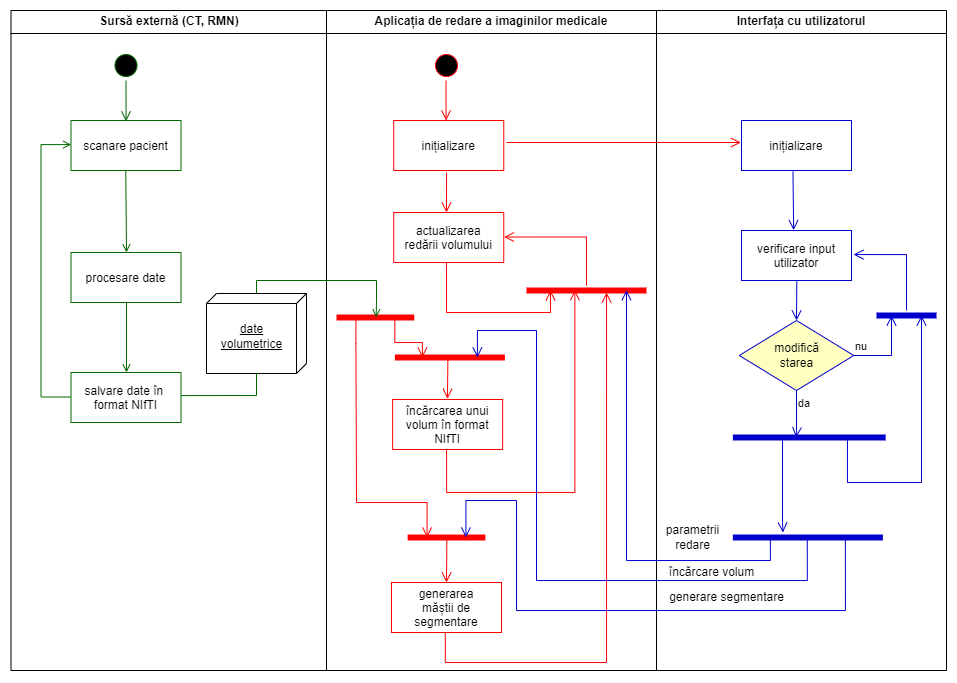
\includegraphics[width=16cm]{images/licenta_activity_diagram.drawio.png}
    \\
    \caption{Diagrama modului de funcționare a aplicației. În stânga este reprezentat modul extern de achiziție a datelor. În centru sunt reprezentate operațiile de bază efectuate de aplicația de redare. În dreapta sunt reprezentate operațiile posibile în interfața cu utilizatorul.}
    \label{fig:app_activity_diagram}
\end{figure}

În figura \ref{fig:app_activity_diagram} sunt prezentate operațiile efectuate în timpul utilizării aplicației. Aceste operații sunt prezentate și sub formă de pseudocod în algoritmul de mai sus. În continuare vor fi prezentate clasele implementate pentru realizarea acestei modalități de funcționare. 

În anexa \hyperref[appendix:1_main_cpp]{1} se găsește punctul de intrare în aplicație, adică funcția main. În același fișier se mai regăsesc și funcții de intializare și logica principală a redării, la cel mai înalt nivel. 

În etapa de inițializare, înainte de crearea ferestrei aplicației, este configurat modul de afișare din glut pentru buffer dublu și RGBA și buffer pentru adâncime. Se creează contextul în care trebuie să funcționeze ImGui și sunt apelate funcțiile pentru initializarea acestuia. Este încărcat modelul de segmentare din LibTorch și sunt stabilite funcțiile care vor fi folosite de către clasa $Interface$ pentru obținerea și manipularea datelor din nivelul aplicației. După care, sunt inițializate matricile $projection$ și $view$ ce vor fi folosite pentru calcularea matricei de transformare $MVP$.

Etapa de redare începe prin curățarea imaginii anterioare de pe ecran și a buffer-ului de culoare și a celui de adâncime. După care este calculată matricea de transformare MVP și încărcată în obiectul shader. De asemenea sunt încărcate și limitele și vectorul de translație pentru AABB. Dacă funcția de transfer a fost schimbată din interfață, aceasta este reîncărcată în obiectul shader. Același fapt este valabil și pentru culorile obiectelor rezultate din segmentarea semantică.

Etapa de afișare a imaginii este încapsulată de apeluri ale unei funcții de obținere a timpului curent în scopul de a calcula timpul necesar afișării unui frame și pentru a limita aplicația la 30 FPS (frame-uri pe secundă) pentru conservarea resurselor.

Clasa $Volume$ are rolul de încărcare a datelor volumetrice într-o textură tridimensională, și de asemenea de a genera texturile necesare pentru funcția de transfer și masca de segmentare. Codul sursă pentru această clasă este în anexele \hyperref[appendix:2_volume_h]{2} și \hyperref[appendix:3_volume_cpp]{3}. 

Citirea datelor volumetrice din memorie este realizată în clasa $Loader$, codul sursă al acesteia fiind în anexele \hyperref[appendix:12_loader_h]{12} și \hyperref[appendix:13_loader_cpp]{13}. Încărcarea datelor volumetrice este realizată în primul rând de către biblioteca nifti. În urma apelului funcției $nifti\_image\_read$ este obținut un bloc continuu de date și informațiile stocate în header-ul fișierului. Tipul de date folosit pentru stocarea volumelor din setul de date CT-ORG este $short$. După ce sunt obținute datele de la clasa Loader, clasa Volume generează texturile necesare pentru datele volumetrice și segmentarea semantică, cea din urma fiind populată ulterior. Parametrii pentru ambele texturi sunt identici, și anume: interpolare liniară a valorilor, și repetarea valorilor de pe margini în afara marginilor. 

Logicile pentru generarea măștii de segmentare și pentru netezirea acesteia sunt încapsulate în clase $thread$ pentru a fi executate în fire de execuție separate de cel principal, deoarece acestea sunt operații complexe cu o durată lungă de timp, iar blocarea interfeței cu utilizatorul și a logicii de redare nu este de dorit. Bineînțeles că în timp ce sunt efectuate aceste operații nu îi mai este permis utilizatorului să înceapă un nou calcul al segmentării sau o nouă netezire a acesteia până la finalizarea celui în curs.

Clasa $Shader$ are rolul de a genera obiectele shader pentru shaderul vertex și cel fragment, și expune o funcție pentru încărcarea logicii acestora din memoria nevolatilă. În această clasă sunt două funcții pentru facilitarea dezvoltării aplicației, anume, pentru detectarea erorilor la compilarea și link-editarea shaderului. Mai sunt expuse și funcții wrapper la cele standard OpenGL, pentru a face mai ușoară încărcarea datelor în obiectele shader. Codul sursă pentru această clasă este în anexele \hyperref[appendix:4_shader_h]{4} și \hyperref[appendix:5_shader_cpp]{5}.

În anexele \hyperref[appendix:6_interface_h]{6} și \hyperref[appendix:7_interface_cpp]{7} sunt definiția și implementarea clasei $Interface$, care este clasa principal responsabilă pentru interfața cu utilizatorul. Această clasă stochează functori care vor fi apelați pentru obținerea și manipularea datelor din aplicație. În acest fel sunt separate responsabilitățile interfeței utilizator și redarea și încărcarea datelor volumetrice. Interfața în sine este prezentată în capitolul \ref{ch:implementation}. Widget-ul folosit pentru modificarea funcției de transfer este $VectorColorPicker$, a cărui cod sursă poate fi găsit în anexele \hyperref[appendix:8_tfwidget_h]{8} și \hyperref[appendix:9_tfwidget_cpp]{9}. În această clasă sunt stocate funcționalități pentru manipularea graficului functei de transfer, afișarea histogramei intensității volumului vizualizat curent și încărcarea și salvarea funcției de transfer din memorie.

Încărcarea modelului de segmentare și funcția pentru folosirea acestuia în scopul generării măștii de segmentare sunt în clasa $PytorchModel$ în anexele \hyperref[appendix:14_ptmodel_h]{14} și \hyperref[appendix:15_ptmodel_cpp]{15}. Funcția $forward$ implementează următorul algoritm:

\begin{enumerate}
    \item Datele stocate într-un $array$ de tip $short$ sunt încărcate într-un obiect Torch $Tensor$ folosind funcția $from\_blob$.
    \item Imaginea volumetrică este interpolată, dimensiunea intrării transformandu-se din $[W, H, D]$\footnote{$W$ = lățimea volumului, $H$ = inailtimea volumului, $D$ = adâncimea volumului} în $[W_I, H_I, D_I$]\footnote{$W_I$, $H_I$. $D_I$ reprezintă dimensiunea la care au fost redimensionate datele în timpul antrenării rețelei neuronale}.
    \item În funcție de valorile $W_P$, $H_P$, $D_P$\footnote{$W_P$, $H_P$, $D_P$ reprezintă dimensiunea peticelor ce au fost folosite la antrenarea modelului, dacă acestea au fost folosite. În mod uzual au fost folosite petice astfel încât imaginea redimensionată să poată fi împărțită în nouda petice disjuncte de aceeași dimensiune (trei pentru fiecare dimensiune)}, imaginea este împărțită în petice disjuncte folosind funcția $split$, acestea fiind pe urmă concatenate pe dimensiunea $batch$ ($B$).
    \item Este obținut rezultatul rețelei neuronale după apelarea funcției $forward$ al acesteia, fiind dat că parametru tensor-ul ce conține peticele concatenate. Astfel intrarea rețelei neuronale are dimensiunea $[B, 1, W_P, H_P, D_P]$, unde $1$ reprezintă numărul de canale, în cazul asta fiind doar luminanță. Ieșirea rețelei neuronale are dimensiunea $[B, L, W_P, H_P, D_P]$, unde $L$ reprezintă numărul de clase de segmentare.
    \item În cazul în care au fost folosite petice, imaginea este recompusă din acestea, rezultând o ieșire de dimensiune $[L, W_P, H_P, D_P]$.
    \item Rezultatul obținut până în acest moment este interpolat pentru a obține o imagine care are dimensiunea celei inițiale, adică $[L, W, H, D]$.
    \item Este aplicată funcția sigmoid pentru rezultatul obținut anterior, folosind un prag de 0.5. Valorile mai mari de acest prag semnifică faptul că voxelul $S_{i, x, y, z}$ aparține clasei de segmentare $L_i$. Astfel sunt obținute $L$ măști de segmentare, câte una pentru fiecare clasă de segmentare.
    \item Măștile de segmentare obținute anterior sunt agregate într-una singură, fiecare element din aceasta putând avea valori de la 0 la $L+1$. Acest rezultat este transformat într-un $array$ de $unsigned char$ folosind funcțiile $contiguous$ și $data\_ptr$. Acesta este rezultatul final returnat de funcția $forward$ a clasei $PytorchModel$.
\end{enumerate}

Intrarea programului este run.py, acesta fiind în anexa \hyperref[appendix:18_run_py]{18}. Se realizează în serie acțiunile marcate ca fiind necesare în configurarea sistemului. Rezultatul fiecărei acțiuni este salvat într-o tabelă de dispersie, și această tabelă este intrare pentru următoarea acțiune, astfel fiind satisfăcute dependențele. Acțiunile posibile implementate în Python sunt enumerate în fișierul jobs.py în anexa \hyperref[appendix:19_jobs_py]{19}, iar fișierele de configurare YAML pentru acestea se află în directorul $config/jobs$ în codul sursă al proiectului și în anexele \hyperref[appendix:37_config_load_data_yaml]{37}, \hyperref[appendix:38_config_load_model_yaml]{38}, \hyperref[appendix:39_config_train_model_yaml]{39}, \hyperref[appendix:40_config_test_model_yaml]{40}, \hyperref[appendix:41_config_deploy_yaml]{41}.


Încărcarea setului de date este realizată într-o clasă ce extinde clasa abstractă $Dataset$ din anexa \hyperref[appendix:23_data_generic_py]{23}, în funcție de fiecare set de date cu care vor fi făcute experimente. Din fișierul de configurare din anexa \hyperref[appendix:33_config_ct_org_yaml]{33} sunt obținute locațiile imaginilor volumetrice și a măștilor de segmentare realizate manual. Pe baza acestora se crează o tabelă de dispersie în care cheia primară reprezintă locația unei imagini și valoarea reprezintă locația măștii de segmentare. Folosind această tabelă de dispersie sunt încărcate datele în instanțe ale clasei $Subject$ din TorchIO. Funcția $get\_data\_loader$ din fișierul loading.py în anexa \hyperref[appendix:27_model_loading_py]{27} împarte setul de date în seturi disjuncte pentru antrenare, validare și testare și întoarce în tabela dependențelor câte un $DataLoader$ pentru fiecare astfel de set.

Antrenarea rețelei neuronale este realizată în funcția $train$ din fișierul train.py din anexa \hyperref[appendix:25_model_train_py]{25}. Valorile funcției cost și ale funcției F1 sunt stocate cu ajutorul unui $SummaryWriter$ pentru a putea fi vizualizate ulterior în Tensorboard. Aceste metrici sunt și afișate la fiecare $metrics\_every$ epoci. În mod asemănător, sunt calculate metrici pentru rețeaua neuronală pe setul de date de validare la fiecare $validate\_every$ epoci. Modelul rezultat poate fi transformat în TorchScript cu funcția $deploy\_model$ din anexa \hyperref[appendix:28_model_deploy_py]{28}. Modulul rezultat este $torchscript\_module\_model.pt$, iar în instanță în care rezultatele antrenării sunt satisfăcătoare, poate fi încărcat în aplicația de redare.
